\documentclass{beamer}
\usepackage{pgfpages}
%\setbeameroption{show notes on second screen=left} %enable for notes
\usepackage{graphicx}
\usepackage{xcolor}
\usepackage{listings}
%\usepackage{transparent}
\usepackage{hyperref}
\lstset{language=python,frame=single}
\usepackage{verbatim}
%\usepackage{apacite}
\usepackage[longnamesfirst]{natbib}
\usepackage{subcaption}
\usepackage{amsmath}
\usepackage{relsize}
\usepackage{appendixnumberbeamer}
\usepackage{xparse}
\usepackage{multimedia}
\usepackage{xcolor}
\usepackage[normalem]{ulem}
\usepackage{tikz}
\usetikzlibrary{matrix,backgrounds}
\usetikzlibrary{positioning}
\usetikzlibrary{shapes,arrows}
\usetikzlibrary{positioning}

\tikzset{onslide/.code args={<#1>#2}{%
  \only<#1>{\pgfkeysalso{#2}} 
}}

\tikzstyle{block} = [rectangle, draw, fill=red!20!blue!10, 
    text width=5em, text centered, rounded corners, minimum height=4em]
\tikzstyle{netnode} = [circle, draw, very thick, inner sep=0pt, minimum size=0.5cm] 
\tikzstyle{relunode} = [rectangle, draw, very thick, inner sep=0pt, minimum size=0.5cm] 
    
\tikzstyle{line} = [draw, line width=1.5pt, -latex']

\pgfdeclarelayer{background}
\pgfsetlayers{background,main}

\pgfdeclarelayer{myback}
\pgfsetlayers{myback,background,main}

\usetheme[numbering=fraction]{metropolis}
\newcommand{\semitransp}[2][35]{\color{fg!#1}#2}

\newcommand\blfootnote[1]{%
  \begingroup
  \renewcommand\thefootnote{}\footnote{#1}%
  \addtocounter{footnote}{-1}%
  \endgroup
}
\renewcommand*\footnoterule{}
%%\AtBeginSection[]
%%{
%%  \begin{frame}
%%    \frametitle{Table of Contents}
%%    \tableofcontents[currentsection]
%%  \end{frame}
%%}

\begin{document}

\title{}
\author{Andrew Lampinen}
\date{FriSem, 5/11/2018}
\frame{\titlepage}

\begin{frame}[standout]
How do humans learn so quickly and effectively? \par
\end{frame}


\begin{frame}{Transfer across domains}
\only<1-2>{
\begin{figure}
\centering
\begin{subfigure}{0.4\textwidth}
\includegraphics[width=\textwidth]{figures/chess_cropped.jpg}
\end{subfigure}%
\begin{subfigure}{0.4\textwidth}
\includegraphics[width=\textwidth]{figures/go.jpg}
\end{subfigure}\\
\uncover<2>{
\begin{subfigure}{0.4\textwidth}
\includegraphics[width=\textwidth]{figures/math.jpg}
\end{subfigure}%
\begin{subfigure}{0.4\textwidth}
\includegraphics[width=\textwidth]{figures/piano.jpg}
\end{subfigure}%
}
\end{figure}
}
\only<3>{
\begin{figure}
\centering
\includegraphics[width=0.8\textwidth]{figures/category_theory.jpg}
\end{figure}
}
\scriptsize
\citep{Lampinen2017a, Hansen2017}
\note{There are deep relationships among the tasks we do -- some are superficially obvious, like Go and Chess, and some are less so, like the mathematical structures underlying music or the fact that we use language to talk about all these domains.\par
Of particular interest to me is deep isomorphisms between mathematical domains, and this is actually one of the things that inspired Gick \& Holyoak.}
\end{frame}

\begin{frame}{Background}
\begin{itemize}
\item Not a new idea: transfer has been called a central component of ``why we're so smart'' \citep{Gentner2003}, and an important source of new ideas \citep{Gick1980}.
\item<2->
However, this perspective has been criticized!\par
\begin{itemize}
\item<3-> ``Significant transfer is probably rare and accounts for very little human behavior. ... We generally do what we have learned to do and no more.'' \citep{Detterman1993}
\end{itemize}
\item<4-> How can we reconcile these different viewpoints?
\end{itemize}
\note{Detterman: ``We generally do what we have learned to do and no more.'' Experimental manipulations in transfer experiments ``have the subtlety of a baseball bat.''\par
Observation from FriSem last year: there is a correlation between the speed of transfer being sought and how important they think it is.}
\end{frame}

\begin{frame}{Transfer speed}
\vspace{1.5em}
I think there's a neglected variable: speed of transfer.\par
\uncover<2->{
\begin{center}
\begin{table}
\begin{tabular}{|c|c|}
\hline
Fast & Slow \\
\hline
\parbox{0.45\textwidth}{
    \begin{itemize}
    \item<2-> one (or a few) examples explicitly shown
    \item<3-> transfer requires explicit awareness of analogy
    \end{itemize}
}
&
\parbox{0.45\textwidth}{
    \begin{itemize}
    \item<2-> learning gradually through many interactions
    \item<3-> {transfer may or may not be explicit}%
               %%\only<4>{\color{red}transfer may or may not be explicit}}
    \end{itemize}
}\\ \hline
\end{tabular}
\end{table}
}
\vspace{1.5em}
\note{E.g. being told about the rules of chess and then seeing if that helps you play go, vs. playing many games of chess and go and seeing if one helps the other}
\end{center}
{
\scriptsize
\citep{Lampinen2017a}
}
\end{frame}

\begin{frame}{Transfer speed and outcomes}
For example, imagine you are about to teach someone to play guitar. Who do you think would likely perform better:
\begin{itemize}
\item a person who has just taken their first piano lesson 
\item a person who has been playing piano for years
\end{itemize}
\begin{figure}
\centering
\begin{subfigure}{0.4\textwidth}
\includegraphics[width=\textwidth]{figures/piano.jpg}
\end{subfigure}~%
\begin{subfigure}{0.4\textwidth}
\includegraphics[width=\textwidth]{figures/guitar.jpg}
\end{subfigure}%
\end{figure}
\note{So transfer may require slow learning in the original domain to set up sufficiently high-quality representations to see an effect}
\end{frame}

\begin{frame}{Transfer speed and opinions}
Transfer speed helps reconcile why some people think transfer is important, while others don't. 
\begin{figure}
\centering
\includegraphics[width=0.5\textwidth]{figures/perspectives_on_transfer.png}
\end{figure}
\end{frame}


\begin{frame}[standout]
Slow transfer between tasks is important.
\end{frame}

\begin{frame}{Abstraction and transfer}
We often progress from procedural to more explicit, abstract, or formal knowledge: \vspace{-0.2em}
\begin{figure}
\centering
\begin{tikzpicture}
\node (img1) {\includegraphics[width=0.33\textwidth]{figures/multiplication_procedural_smaller.png}};
\uncover<2->{
\node (img2) at ([yshift=-2em]img1.east) {\includegraphics[width=0.33\textwidth]{figures/factoring_polynomial_worksheet.png}};
}
\uncover<3->{
\node (img3) at ([yshift=-3em]img2.east) {\includegraphics[width=0.5\textwidth]{figures/prime_ideals.png}};
}
\end{tikzpicture}
\end{figure}\vspace{-0.2em}
\uncover<4>{These are related tasks that share some structure! Is it useful to think about this from the perspective of transfer?}
\note{worksheetfun.com\par
Less abstract and more abstract reasoning can be seen as partially distinct tasks that share some common structure. There are different ways that procedural knowledge could support more formal, setting up representations and intuitions, having examples to reason over, ...}
\end{frame}

\begin{frame}{Is abstraction transfer?}
Yet there are also times when procedural and formal knowledge seem partially dissociable:
\begin{figure}
\centering
\begin{subfigure}{0.4\textwidth}
\includegraphics[width=\textwidth]{figures/piano.jpg}
\end{subfigure}~%
\begin{subfigure}{0.5\textwidth}
\includegraphics[width=\textwidth]{figures/mixolydian.png}
\end{subfigure}%
\end{figure}
\note{}
\end{frame}

\begin{frame}[standout]
When and how do procedural and more explicit, abstract, or formal knowledge influence each other?
\end{frame}

\begin{frame}<-8>[label=phenomena]
\frametitle<-9>{A diagram of potential phenomena of interest}
\frametitle<10>{What explicit knowledge?}
\vspace{-1em}
\begin{figure}
\centering
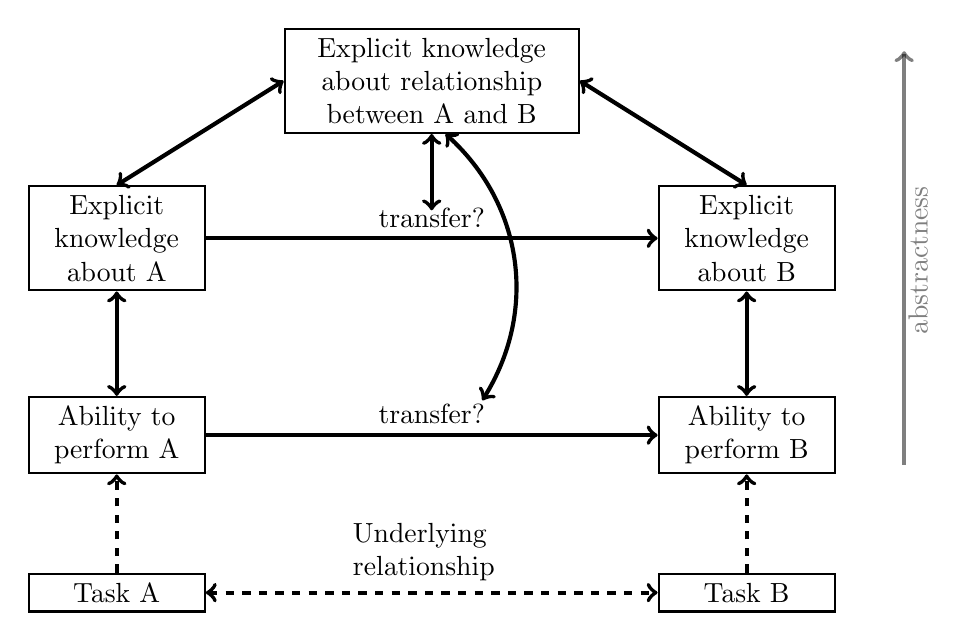
\begin{tikzpicture}[auto] %% TODO? highlighting
\node [rectangle, draw, thick, text width=2cm, align=center, onslide={<10>,{opacity=0.2}}] (A) at (-4, 0) {Task A}; 
\node [rectangle, draw, thick, text width=2cm, align=center, onslide={<10>,{opacity=0.2}}] (B) at (4, 0) {Task B}; 
\path [line, dashed, <->, onslide={<10>,{opacity=0.2}}] (A.east) to node[text width=2cm] (underlying) {Underlying relationship} (B.west); 

\uncover<2->{
\node [rectangle, draw, thick, text width=2cm, align=center, onslide={<10>,{opacity=0.2}}] (Aproc) at (-4, 2) {Ability to perform  A}; 
\node [rectangle, draw, thick, text width=2cm, align=center, onslide={<10>,{opacity=0.2}}] (Bproc) at (4, 2) {Ability to perform B}; 
\path [line, ->, dashed, onslide={<10>,{opacity=0.2}}] (A.north) to  node (Atrans) {}(Aproc.south); 
\path [line, ->, dashed, onslide={<10>,{opacity=0.2}}] (B.north) to node (Btrans) {} (Bproc.south); 
}

\uncover<3->{
\path [line, ->, onslide={<10>,{opacity=0.2}}] (Aproc.east) to node (proctrans) {transfer?} (Bproc.west); 
}

\uncover<4->{
\node [rectangle, draw, thick, text width=2cm, align=center] (Aabs) at (-4, 4.5) {Explicit knowledge about A}; 
\node [rectangle, draw, thick, text width=2cm, align=center] (Babs) at (4, 4.5) {Explicit knowledge about B}; 
\path [line, <->, onslide={<10>,{opacity=0.2}}] (Aproc.north) to  node (Atrans) {}(Aabs.south); 
\path [line, <->, onslide={<10>,{opacity=0.2}}] (Bproc.north) to node (Btrans) {} (Babs.south); 
}
\uncover<5->{
\path [line, ->, onslide={<10>,{opacity=0.2}}] (Aabs.east) to node (abstrans) {transfer?} (Babs.west); 
}
\uncover<6->{
\node [rectangle, draw, thick, text width=3.5cm, align=center] (ABabs) at (0, 6.5) {Explicit knowledge about relationship between A and B}; 
}
\uncover<7->{
\path [line, <->, onslide={<10>,{opacity=0.2}}] (Aabs.north) to  (ABabs.west); 
\path [line, <->, onslide={<10>,{opacity=0.2}}] (Babs.north) to  (ABabs.east); 
\path [line, <->, onslide={<10>,{opacity=0.2}}] ([yshift=-0.5em]abstrans.north) to(ABabs.south); 
\path [line, <->, bend right=40, onslide={<10>,{opacity=0.2}}] ([xshift=-0.5em, yshift=-0.25em]proctrans.north east) to([xshift=0.5em]ABabs.south); 
}
\uncover<8->{
\node (abs0) at (6, 1.5) {};
\node (abs1) at (6, 7) {};
\path [line, ->, opacity=0.5] (abs0) to node [xshift=0.5em, yshift=3em, opacity=0.5, rotate=90] {abstractness} (abs1); 
}

\end{tikzpicture}
\end{figure}

\end{frame}

\section{Experiment design}

\begin{frame}<-2>[label=exp_des]{Experiment design}
\only<4->{
\vspace{-1em}
}
\begin{figure}
\centering
\begin{tikzpicture}[auto] 
\node (time00) at (-2, -1) {};
\node (time01) at (5, -1) {};
\node [rectangle, draw, thick, text width=2cm, minimum height=1.5cm, align=center ] (A) at (0, 0) {
    \only<-2>{Task A}
    \only<3->{\includegraphics[width=2cm]{figures/door_example.png}}}; 

\node [rectangle, draw, thick, text width=2cm, minimum height=1.5cm, align=center] (B) at (3, 0) {
    \only<-2>{Task B}
    \only<3->{\includegraphics[width=2cm]{figures/fractal_example.png}}};
\path [line, ->] (time00) to (time01); 

\only<2->{
\node (sess1) at (-2.5, 0) {\bf Day 1};

\node (sess2) at (-2.5, -2.5) {\bf Day 2};
\node (time10) at (-2, -3.5) {};
\node (time11) at (5, -3.5) {};
\node [rectangle, draw, thick, text width=2cm, minimum height=1.5cm, align=center ] (A1) at (0, -2.5) {
    \only<-2>{Task A}
    \only<3->{\includegraphics[width=2cm]{figures/door_example.png}}};
\node [rectangle, draw, thick, text width=2cm, minimum height=1.5cm, align=center] (B1) at (3, -2.5) {
    \only<-2>{Task B}
    \only<3->{\includegraphics[width=2cm]{figures/fractal_example.png}}};
\path [line, ->] (time10) to (time11); 

\node (sess1) at (-2.5, -5) {\bf Day 3};
\node (time20) at (-2, -6) {};
\node (time21) at (5, -6) {};
\node [rectangle, draw, thick, text width=2cm, minimum height=1.5cm, align=center ] (A2) at (0, -5) {
    \only<-2>{Task A}
    \only<3->{\includegraphics[width=2cm]{figures/door_example.png}}};
\node [rectangle, draw, thick, text width=2cm, minimum height=1.5cm, align=center] (B2) at (3, -5) {
    \only<-2>{Task B}
    \only<3->{\includegraphics[width=2cm]{figures/fractal_example.png}}}; 
}

\only<2-3>{
\path [line, ->] (time20) to (time21); 
}

\only<4->{
\node (time22) at (8, -6) {};
\node [rectangle, draw, thick, text width=2cm, minimum height=1.5cm, align=center] (B2) at (6, -5) {Explicit knowledge?}; 
\path [line, ->] (time20) to (time22); 
}
\end{tikzpicture}
\end{figure}
\end{frame}

\begin{frame}{Tasks}
\only<1>{
\url{https://web.stanford.edu/~lampinen/mturk/il/web/experiment_mockup.html}
}
\only<2->{
\begin{figure}
\centering
\begin{subfigure}{0.45\textwidth}
\includegraphics[width=\textwidth]{figures/door_example.png}
\end{subfigure}~
\begin{subfigure}{0.45\textwidth}
\includegraphics[width=\textwidth]{figures/fractal_example.png}
\end{subfigure}\\
\begin{subfigure}[b]{0.45\textwidth}
\vspace{0.5em}
\centering
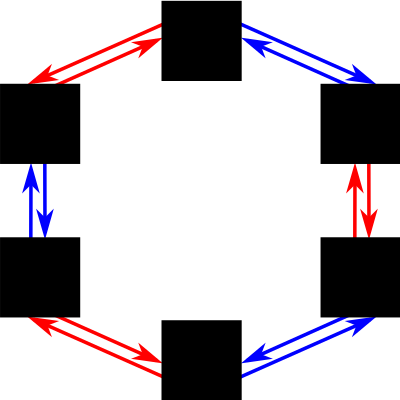
\includegraphics[width=0.8\textwidth]{../../diagrams/hexagon_bi.png}
\end{subfigure}~
\begin{subfigure}[b]{0.45\textwidth}
\vspace{0.5em}
\centering
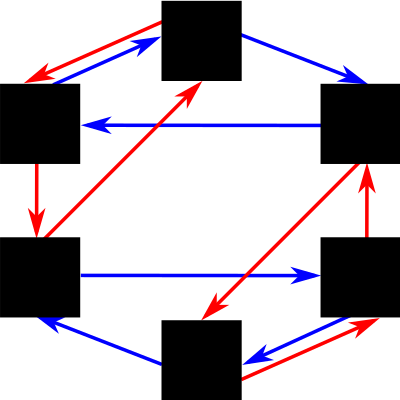
\includegraphics[width=0.8\textwidth]{../../diagrams/hexagon_tri.png}
\end{subfigure}
\end{figure}}
\note{experimental manipulation will be which structure they have in the fractal condition, whether it's the same as door, and outcomes will be performance in fractal condition and abstractions.}
\end{frame}

\begin{frame}[label=structure_diagrams]{Structures}
\begin{center}
\begin{table}
\begin{tabular}{|c|c|}
\hline
Flipping & Cycling \\
\hline
\parbox{0.45\textwidth}{
\begin{figure}
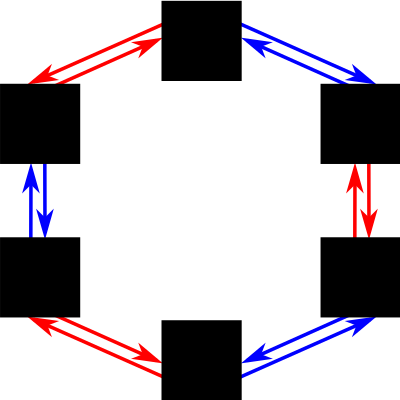
\includegraphics[width=0.35\textwidth]{../../diagrams/hexagon_bi.png}
\end{figure}
}
&
\parbox{0.45\textwidth}{
\begin{figure}
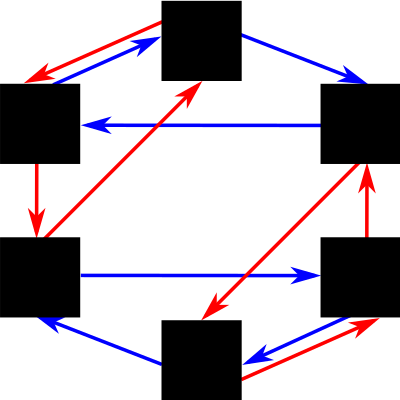
\includegraphics[width=0.35\textwidth]{../../diagrams/hexagon_tri.png}
\end{figure}
}\\ \hline
\end{tabular}
\end{table}
\end{center}
\begin{itemize}
\item<2> Balanced for average path length, number of actions entering/exiting a room, etc.
\end{itemize}
\end{frame}

\begin{frame}{\(2 \times 2\)}
\begin{center}
\begin{table}
\begin{tabular}{|r|c|c|}
\hline
& \multicolumn{2}{|c|}{Fractal structure} \\
& \multicolumn{1}{|c}{Flipping} & \multicolumn{1}{c|}{Cycling} \\
\hline
Isomorphic
&
\parbox{0.3\textwidth}{
\vspace{0.1em}
\includegraphics[width=0.15\textwidth]{figures/door_example.png}~%
\includegraphics[width=0.15\textwidth]{figures/fractal_example.png}\\
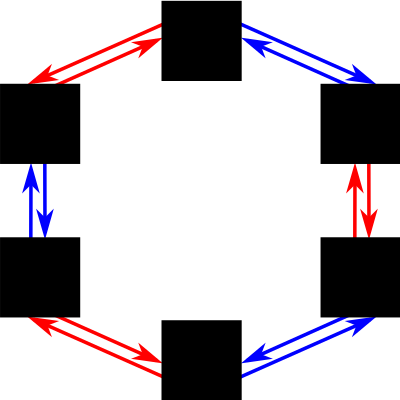
\includegraphics[width=0.15\textwidth]{../../diagrams/hexagon_bi.png}~%
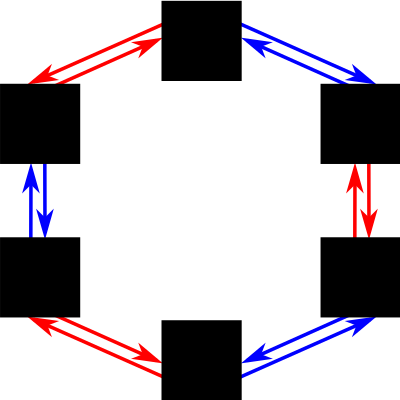
\includegraphics[width=0.15\textwidth]{../../diagrams/hexagon_bi.png}
\vspace{0.1em}
}
&
\parbox{0.3\textwidth}{
\vspace{0.1em}
\includegraphics[width=0.15\textwidth]{figures/door_example.png}~%
\includegraphics[width=0.15\textwidth]{figures/fractal_example.png}\\
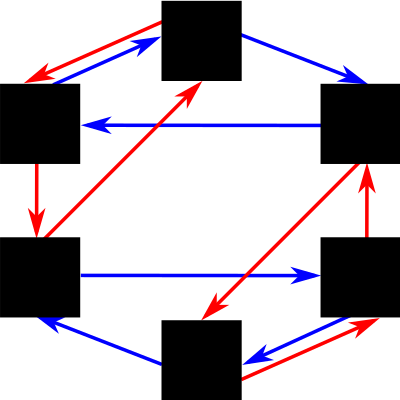
\includegraphics[width=0.15\textwidth]{../../diagrams/hexagon_tri.png}~%
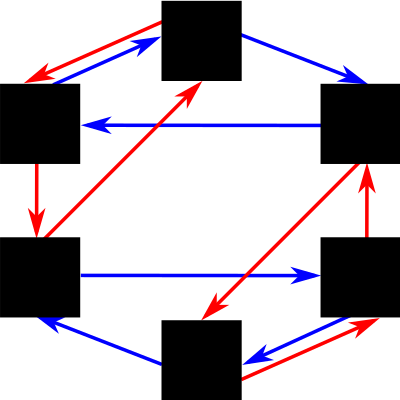
\includegraphics[width=0.15\textwidth]{../../diagrams/hexagon_tri.png}
\vspace{0.1em}
}
\\\hline
Non-isomorphic
&
\parbox{0.3\textwidth}{
\vspace{0.1em}
\includegraphics[width=0.15\textwidth]{figures/door_example.png}~%
\includegraphics[width=0.15\textwidth]{figures/fractal_example.png}\\
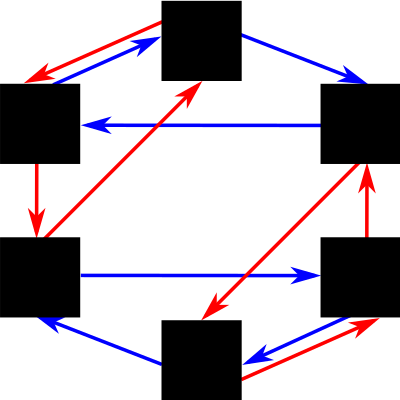
\includegraphics[width=0.15\textwidth]{../../diagrams/hexagon_tri.png}~%
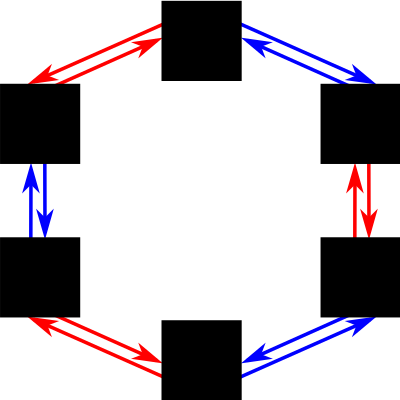
\includegraphics[width=0.15\textwidth]{../../diagrams/hexagon_bi.png}
\vspace{0.1em}
}
&
\parbox{0.3\textwidth}{
\vspace{0.1em}
\includegraphics[width=0.15\textwidth]{figures/door_example.png}~%
\includegraphics[width=0.15\textwidth]{figures/fractal_example.png}\\
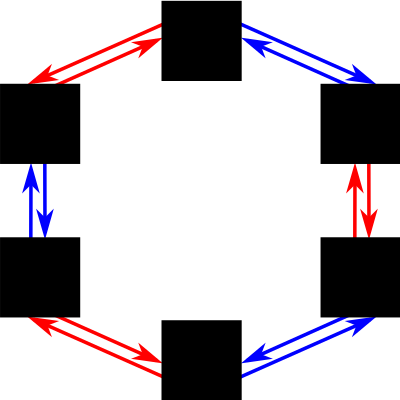
\includegraphics[width=0.15\textwidth]{../../diagrams/hexagon_bi.png}~%
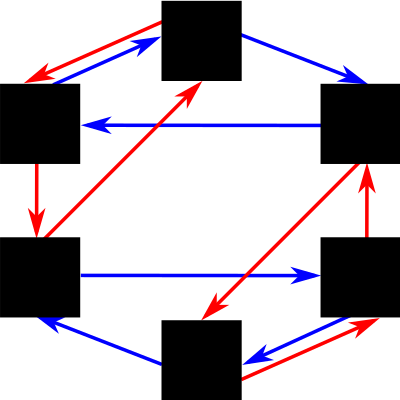
\includegraphics[width=0.15\textwidth]{../../diagrams/hexagon_tri.png}
\vspace{0.1em}
}
\\  \hline
\end{tabular}
\end{table}
\end{center}
\end{frame}

\againframe<3-4>{exp_des}
\againframe<10>{phenomena}

\begin{frame}{Explicit knowledge about a single task}
Within fractals:
\begin{figure}
\centering
\begin{subfigure}{0.45\textwidth}
\includegraphics[width=\textwidth]{figures/diagram_selection_example.png}
\end{subfigure}~
\begin{subfigure}{0.45\textwidth}
\includegraphics[width=\textwidth]{figures/drag_drop_example.png}
\end{subfigure}
\end{figure}
\end{frame}

\begin{frame}{Explicit awareness of a relationship between tasks}
\begin{figure}
\centering
\begin{subfigure}{0.9\textwidth}
\includegraphics[width=\textwidth]{figures/correspondence_suspect.png}
\end{subfigure}\\
\begin{subfigure}{0.9\textwidth}
\includegraphics[width=\textwidth]{figures/one_task_helpful.png}
\end{subfigure}
\end{figure}
\end{frame}

\begin{frame}{Explicit identification of the mapping between tasks}
\begin{figure}
\centering
\begin{subfigure}{0.45\textwidth}
\includegraphics[width=\textwidth]{figures/corr_drag_drop.png}
\end{subfigure}~
\begin{subfigure}{0.45\textwidth}
\includegraphics[width=\textwidth]{figures/corr_ident.png}
\end{subfigure}
\end{figure}
\end{frame}

\begin{frame}{Interrogating explicit knowledge}
\begin{itemize}
\item It's difficult to assess whether knowledge is explicit or implicit \citep{Newell2014} -- results can be altered by the details of the probe. 
\item<2-> We carefully developed our protocol, including: 
\begin{itemize}
\item<3-> Asking within-task explicit knowledge questions only on one task, and before any between-task questions.
\item<4-> Organizing questions in order of increasing specificity. 
\end{itemize}
\item <5-> However, likely needs more work, input is welcome.
\end{itemize}
\end{frame}

\begin{frame}<1-5>[label=res_ques]{Research questions}
\begin{itemize}
\item Does isomorphism affect task performance? 
    \only<7->{
    \begin{itemize}
    \item[] {\bf Yes.}
    \end{itemize}}
\item<2->
    \only<6>{\semitransp[20]{What affects within-task explicit knowledge?}}%
    \only<2-5,7->{What affects within-task explicit knowledge?}%
    \only<8->{
    \begin{itemize}
    \item[] {\bf Performance, isomorphism(?)} 
    \end{itemize}}
\item<3->
    \only<6-7>{\semitransp[20]{What affects awareness of the relationship between the tasks?}}%
    \only<3-5,8->{What affects awareness of the relationship between the tasks?}%
    \only<9->{
    \begin{itemize}
    \item[] {\bf Isomorphism, structure, performance} 
    \end{itemize}}
\item<4->
    \only<6-8>{\semitransp[20]{What affects ability to explicitly identify the relationship?}}%
    \only<4-5,9->{What affects ability to explicitly identify the relationship?}%
    \only<10->{
    \begin{itemize}
    \item[] {\bf Performance?} 
    \end{itemize}}
\item<5->
    \only<6-9>{\semitransp[20]{Is awareness related to transfer?}}%
    \only<5,10->{Is awareness related to transfer?}%
    \only<11->{Maybe, but it is not determinative.}
\end{itemize}
\end{frame}

\section{Results}

\againframe<6>{res_ques}

\begin{frame}<1>[label=iso_bet_B]{Subjects in isomorphic condition perform better at fractals}
\begin{figure}
\centering
\only<1>{
\includegraphics[width=0.9\textwidth]{figures/ex3/ns_more_basic_plot_fractal.png}
}\only<2>{
\includegraphics[width=0.9\textwidth]{figures/ex3/ns_by_correspondence_suspect.png}
}\only<3> {
\includegraphics[width=0.9\textwidth]{figures/ex3/ns_by_en.png}
}\only<4> {
\includegraphics[width=0.9\textwidth]{figures/ex3/ns_by_sl.png}
} \only<5> {
\includegraphics[width=0.9\textwidth]{figures/ex3/ns_by_oth.png}
} \only<6> {
\includegraphics[width=0.9\textwidth]{figures/ex3/ns_by_oth_T.png}
}
\end{figure}
{\scriptsize Error bars represent 95\%-confidence intervals}
\end{frame}

\begin{frame}{True in both structures}
\begin{figure}
\centering
\includegraphics[width=0.9\textwidth]{figures/ex3/ns_basic_plot_fractal.png}
\end{figure}
{\scriptsize Error bars represent 95\%-confidence intervals}
\end{frame}

\begin{frame}{No effect on door performance}
\begin{figure}
\centering
\includegraphics[width=0.9\textwidth]{figures/ex3/ns_more_basic_plot_door.png}
\end{figure}
{\scriptsize Error bars represent 95\%-confidence intervals}
\end{frame}

\begin{frame}[standout]
Isomorphism improves performance on fractals.
\end{frame}

\againframe<7>{res_ques}

\begin{frame}
Note: we have much less power to detect explicit effects, because they're generally based off of one answer per question per subject in only the final session.
\end{frame}

\begin{frame}{Better performance on task predicts better mapping}
\begin{figure}
\centering
\only<1>{
    \includegraphics[width=0.8\textwidth]{figures/drag_drop_example.png}
} \only<2>{
    \includegraphics[width=\textwidth]{figures/ex3/nac_by_ns.png}
}
\end{figure}
\end{frame}


\begin{frame}<-3>[label=iso_within_task]{Isomorphism may influence ability to identify structure}
\begin{figure}
\centering
\only<1>{
    \includegraphics[height=0.9\textheight]{figures/diagram_selection_example.png}
} \only<2>{
    \includegraphics[width=0.9\textwidth]{figures/ex3/ds_by_iso.png}
}\only<3>{
    \includegraphics[width=0.9\textwidth]{figures/ex3/ds_by_iso_by_group.png}
}\only<4>{
    \includegraphics[width=0.9\textwidth]{figures/ex3/ds_by_iso_by_cs.png}
} \only<5> {
    \includegraphics[width=0.9\textwidth]{figures/ex3/ds_by_iso_by_en.png}
} \only<6> {
    \includegraphics[width=0.9\textwidth]{figures/ex3/ds_by_iso_by_oth.png}
}

\end{figure}
\uncover<2->{\scriptsize Error bars represent bootstrap 95\%-confidence intervals}
\end{frame}

\begin{frame}<-2>[label=iso_within_nac]{Isomorphism may influence mapping of structure}
\begin{figure}
\centering
\only<1>{
    \includegraphics[height=0.9\textheight]{figures/drag_drop_example.png}
} \only<2>{
    \includegraphics[width=0.9\textwidth]{figures/ex3/nac_by_iso_by_group.png}
} \only<3>{
    \includegraphics[width=0.9\textwidth]{figures/ex3/nac_by_iso_group_cs.png}
} \only<4>{
    \includegraphics[width=0.9\textwidth]{figures/ex3/nac_by_iso_oth.png}
}
\end{figure}
\uncover<2->{\scriptsize Error bars represent bootstrap 95\%-confidence intervals}
\end{frame}

\begin{frame}[standout]
Isomorphism may improve explicit knowledge about fractals.
\end{frame}

\againframe<8>{res_ques} % Awareness

\begin{frame}{Similarity ratings}
\begin{figure}
\centering
\only<1>{
    \includegraphics[width=0.9\textwidth]{figures/similarity_likert.png}
}
\only<2>{
    \includegraphics[width=0.9\textwidth]{figures/ex3/sl_by_iso.png}
}
\only<3>{
    \includegraphics[width=0.9\textwidth]{figures/ex3/sl_by_iso_ns.png}
}
\end{figure}
\uncover<2->{\scriptsize Error bars represent 95\%-confidence intervals}
\end{frame}

\begin{frame}{Suspect correspondence?}
\begin{figure}
\centering
\only<1>{
    \includegraphics[width=0.9\textwidth]{figures/correspondence_suspect.png}
}
\only<2>{
    \includegraphics[width=0.9\textwidth]{figures/ex3/cs_by_iso.png}
}
\only<3>{
    \includegraphics[width=0.9\textwidth]{figures/ex3/cs_by_iso_group.png}
}
\end{figure}
\uncover<2->{\scriptsize Error bars represent 95\%-confidence intervals}
\end{frame}

\begin{frame}{One task helpful for other?}
\begin{figure}
\centering
\only<1>{
    \includegraphics[width=0.9\textwidth]{figures/one_task_helpful.png}
}
\only<2>{
    \includegraphics[width=0.9\textwidth]{figures/ex3/oth_by_iso.png}
}
\only<3>{
    \includegraphics[width=0.9\textwidth]{figures/ex3/oth_by_iso_ns.png}
}
\end{figure}
\uncover<2->{\scriptsize Error bars represent 95\%-confidence intervals}
\end{frame}

\begin{frame}[standout]
Subjects in the isomorphic condition were more likely to notice the relationship between the tasks, especially if they performed well.
\end{frame}

\againframe<9>{res_ques} % identification 

\begin{frame}
Note: we have even less power here because analyses only make sense for subjects in the isomorphic condition, and in this experiment we collected this data only a subset of subjects.
\end{frame}

\begin{frame}<-2>[label=cddnac]{Subjects can explicitly identify mapping better than chance}
\begin{figure}
\centering
\only<1>{
    \includegraphics[height=0.9\textheight]{figures/corr_drag_drop.png}
} \only<2>{
    \includegraphics[width=0.9\textwidth]{figures/ex3/cddnac_only_iso.png}
} \only<3>{
    \includegraphics[width=0.9\textwidth]{figures/ex3/cddnac_by_group_cs.png}
} \only<4>{
    \includegraphics[width=0.9\textwidth]{figures/ex3/cddnac_isoonly_by_oth.png}
}
\end{figure}
\uncover<2->{\scriptsize Error bars represent 95\%-confidence intervals}
\note{< 40 subjects in this, < 20 s in isomorphic condition...}
\end{frame}

\begin{frame}{Only weakly related to performance}
\begin{figure}
\centering
    \includegraphics[width=0.9\textwidth]{figures/ex3/cddnac_only_iso_by_ns.png}
\end{figure}
{\scriptsize Error bars represent 95\%-confidence intervals}
\end{frame}

\begin{frame}[standout]
Subjects could identify the relationship somewhat above chance, weakly predicted by performance.
\end{frame}

\againframe<10>{res_ques} % Awareness -> ?

\begin{frame}{Assessing awareness}
\begin{figure}
\centering
\includegraphics[width=0.8\textwidth]{figures/similarity_likert.png}\\
\includegraphics[width=0.8\textwidth]{figures/correspondence_suspect.png}\\
\includegraphics[width=0.8\textwidth]{figures/one_task_helpful.png}
\end{figure}
\note{Also asked some free response which I haven't looked at too thoroughly yet}
\end{frame}

\againframe<1-6>{iso_bet_B}

\begin{frame}{Awareness}
\begin{itemize}
\item Most measure of awareness are not associated with basic transfer.
\item<2-> One task helpful for other ratings, however, appear to be.
\item<3-> This pattern was similar for other awareness analyses, so we'll focus on one-task-helpful from now on.
\end{itemize}
\end{frame}

\againframe<1-2,6>{iso_within_task}

\againframe<1-2,4>{iso_within_nac}

\againframe<1-2,4>{cddnac}

\begin{frame}{What's up with ``one task helpful for other?''}
\begin{figure}
\centering
\includegraphics[width=0.8\textwidth]{figures/one_task_helpful.png}
\end{figure}
\vspace{-1em}
\begin{itemize}
\item<2-> Isomorphism still significantly reduced average number of steps even among those who gave low ratings (though the effect was smaller).
\item<3-> Similar on explicit within-task questions (trending on diagram selection, significant on fractal assignments). 
\item<4-> This question was asked \textbf{after} the similarity, suspect, and noticed questions, \textbf{and} immediately after asking subjects to describe a correspondence.
\end{itemize}
\end{frame}

\begin{frame}[standout]
Awareness appears to be neither necessary nor sufficient for transfer, but may be positively asssociated with it. 
\end{frame}


\begin{frame}{Conclusions}
\begin{itemize}
\item We see evidence of slow transfer between tasks.
\item<2-> This also appears to increase explicit within-task knowledge. 
\item<3-> This transfer may not require awareness, though awareness may be positively associated with it. 
\end{itemize}
\end{frame}

\begin{frame}{Next steps \& possible future directions}
\begin{itemize}
\item See whether these results hold/replicate 
\item<2-> Verify that direction of transfer is caused by order and not e.g. grounding
\item<3-> Include distractor tasks between
\item<4-> Integrating abstractions (either taught or interrogated) earlier on one or both tasks
\item<5-> Try to model this with a neural network
\end{itemize}
\end{frame}

\begin{frame}{Acknowledgements}
\vspace{-2em}
\begin{figure}
\centering
\begin{tikzpicture}[auto] 
\node at (0, 0) {\includegraphics[width=2cm]{figures/people/jay.jpg}};
\node at (2, 0) {\includegraphics[width=2cm]{figures/people/arianna.jpg}};
\node at (4, 0) {\includegraphics[width=2cm]{figures/people/katherine.jpg}};
\node at (7, 0) {\includegraphics[width=2cm]{figures/people/erin.jpg}};
\node at (9, 0) {\includegraphics[width=2cm]{figures/people/yochai.jpg}};
\node at (7, -2) {\includegraphics[width=2cm]{figures/people/jesse.jpg}};
\node at (9, -2) {\includegraphics[width=2cm]{figures/people/pam.jpg}};
\node at (8, -5) {\includegraphics[width=2cm]{figures/nsf.jpeg}};

\node at (0, -3) {\includegraphics[width=1.5cm]{figures/people/dan.jpg}};
\node at (1.5, -3) {\includegraphics[width=1.5cm]{figures/people/mona.jpg}};
\node at (3, -3) {\includegraphics[width=1.5cm]{figures/people/corey.jpg}};
\node at (4.5, -3) {\includegraphics[width=1.5cm]{figures/people/robert.jpg}};
\node at (0, -4.5) {\includegraphics[width=1.5cm]{figures/people/dawn.jpg}};
\node at (1.5, -4.5) {\includegraphics[width=1.5cm]{figures/people/daniel.jpg}};
\node at (3, -4.5) {\includegraphics[width=1.5cm]{figures/people/tyler.png}};
\node at (4.5, -4.5) {\includegraphics[width=1.5cm]{figures/people/pam.jpg}};
\node at (0, -6) {\includegraphics[width=1.5cm]{figures/people/erin.jpg}};
\node at (1.5, -6) {\includegraphics[width=1.5cm]{figures/people/shaw.jpg}};
\node at (6, -6) {\bf You!};

\end{tikzpicture}
\end{figure}
\end{frame}

\begin{frame}[allowframebreaks]
\bibliographystyle{plainnat}
\blfootnote{\bibliography{transfer}}
\end{frame}

\appendix

\againframe<1>{structure_diagrams}

\begin{frame}{Alternation}
\begin{figure}
\centering
\only<1>{
    \includegraphics[width=0.9\textwidth]{figures/ex3/alt_fractal_by_group.png}
} \only<2>{
    \includegraphics[width=0.9\textwidth]{figures/ex3/alt_door_by_group.png}
}
\end{figure}
{\scriptsize Error bars represent 95\%-confidence intervals}
\end{frame}

\againframe<1>{structure_diagrams}

\begin{frame}{Cycling}
\begin{figure}
\centering
\only<1>{
    \includegraphics[width=0.9\textwidth]{figures/ex3/cyc_fractal_by_group.png}
} \only<2>{
    \includegraphics[width=0.9\textwidth]{figures/ex3/cyc_door_by_group.png}
}
\end{figure}
{\scriptsize Error bars represent 95\%-confidence intervals}
\end{frame}

\begin{frame}{Policies}
\begin{itemize}
\item The remaining analyses rely on the idea of a \emph{policy} from reinforcement learning.
\item<2-> A policy is a function that maps states to action probabilities:
\begin{center}
\begin{table}

\begin{tabular}{|c|c|c|}
\hline 
& \(P\)(Acid) & \(P\)(Ray) \\
\hline
\includegraphics[width=0.25\textwidth]{figures/fractal_example.png} & 0.75 & 0.25\\ \hline
\includegraphics[width=0.25\textwidth]{figures/fractal_example_2.png} & 0.5 & 0.5 \\ \hline
\end{tabular}
\end{table}
\end{center}
\end{itemize}
\end{frame}

\begin{frame}{Policy alignment}
\begin{itemize}
\item How similar is participants behavior between the tasks? 
\item<2-> We'll quantify this by looking at similarity between their policies.
\begin{columns}
\begin{column}{0.5\textwidth}
\begin{center}
\begin{tabular}{|c|c|c|}
\hline 
& \(P\)(Acid) & \(P\)(Ray) \\
\hline
\includegraphics[width=0.25\textwidth]{figures/fractal_example.png} & 0.75 & 0.25\\ \hline
\includegraphics[width=0.25\textwidth]{figures/fractal_example_2.png} & 0.5 & 0.5 \\ \hline
 \vdots & \vdots & \vdots \\ \hline
\end{tabular}
\end{center}
\end{column}
\begin{column}{0.5\textwidth}
\begin{center}
\begin{tabular}{|c|c|c|}
\hline 
& \(P\)(Right) & \(P\)(Left) \\
\hline
\includegraphics[width=0.25\textwidth]{figures/door_example_3.png} & 0.5 & 0.5\\ \hline
\includegraphics[width=0.25\textwidth]{figures/door_example_2.png} & 0.75 & 0.25 \\ \hline
 \vdots & \vdots & \vdots \\ \hline
\end{tabular}
\end{center}
\end{column}
\end{columns}
\item<3-> We'll consider all the structure-preserving mappings between the door and fractal policies, and see how well the participants' policies align across tasks.
\end{itemize}
\end{frame}

\begin{frame}{Policy alignment is greater in isomorphic condition}
\begin{figure}
\centering
\includegraphics[width=0.9\textwidth]{figures/ex3/distributional_similarities_by_isomorphic.png}
\end{figure}
{\scriptsize Error bars represent bootstrap 95\%-confidence intervals}
\note{Not too surprising, would be true if people were learning the tasks sufficiently well even if they treated them completely independently}
\end{frame}

\begin{frame}{Policy alignment is related to performance}
\begin{figure}
\centering
\only<1>{
\includegraphics[width=0.9\textwidth]{figures/ex3/ns_by_minl1_iso.png}
}
\only<2>{
\includegraphics[width=0.9\textwidth]{figures/ex3/ns_by_minl1_iso_group.png}
}
\end{figure}
{\scriptsize Error bars represent 95\%-confidence intervals}
\note{Some subjects in the *non*-isomorphic condition appear to be trying to transfer, and doing worse because of it!}
\end{frame}

%%\begin{frame}{Not a consciousness effect?}
%%\begin{figure}
%%\centering
%%\includegraphics[width=0.9\textwidth]{figures/ex3/ns_by_minl1_iso_cs.png}
%%\end{figure}
%%{\scriptsize Error bars represent 95\%-confidence intervals}
%%\end{frame}
%%
%%\begin{frame}[standout]
%%Policy alignment strongly affects performance. \par
%%\uncover<2->{
%%\vspace{1em}
%%Some subjects may be ``trying'' to transfer in the non-isomorphic condition, and actually be harmed by it!
%%}
%%\end{frame}


\begin{frame}{Suggestive but not significant}
\only<1>{
\includegraphics[width=0.9\textwidth]{figures/corr_ident.png}
} \only<2> {
\includegraphics[width=0.9\textwidth]{figures/ex3/imp_vs_exp_swaps.png}
} \only<3> {
\centering
\resizebox{!}{0.4\textheight}{%
% Table created by stargazer v.5.2 by Marek Hlavac, Harvard University. E-mail: hlavac at fas.harvard.edu
% Date and time: Fri, May 11, 2018 - 02:36:12 PM
\begin{tabular}{@{\extracolsep{5pt}}lc} 
\\[-1.8ex]\hline 
\hline \\[-1.8ex] 
\\[-1.8ex] & correspondence\_swaps \\ 
\hline \\[-1.8ex] 
 best\_explicit\_mapping\_swaps & $-$0.081 (1.204) \\ 
  & t = $-$0.067 \\ 
  & p = 0.947 \\ 
  best\_implicit\_mapping\_swaps & 2.086 (1.279) \\ 
  & t = 1.631 \\ 
  & p = 0.103 \\ 
  Constant & 0.030 (0.839) \\ 
  & t = 0.036 \\ 
  & p = 0.972 \\ 
 \hline \\[-1.8ex] 
Observations & 17 \\ 
Log Likelihood & $-$8.682 \\ 
Akaike Inf. Crit. & 23.365 \\ 
\hline 
\hline \\[-1.8ex] 
\textit{Note:}  & \multicolumn{1}{r}{$^{*}$p$<$0.1; $^{**}$p$<$0.05; $^{***}$p$<$0.01} \\ 
\end{tabular} 
}}
\end{frame}

\begin{frame}
\begin{figure}
\centering
\includegraphics[width=\textwidth]{figures/ex3/policy_tsne.png}
\end{figure}
\end{frame}

\begin{frame}{Flipping is easier}
\begin{figure}
\centering
\includegraphics[width=0.9\textwidth]{figures/ex3/flipping_easier.png}
\end{figure}
{\scriptsize Error bars represent 95\%-confidence intervals}
\end{frame}

\begin{frame}
\begin{figure}
\centering
\includegraphics[width=0.9\textwidth]{figures/ex3/ns_individual_curve_plot.png}
\end{figure}
{\scriptsize Error bars represent 95\%-confidence intervals}
\end{frame}

\againframe<1-2,4-5>{iso_within_task}

\againframe<3>{iso_within_nac}

\againframe<3>{cddnac}

\begin{frame}{Models: Number of steps needed on fractal trials}
\begin{center}
\resizebox{!}{0.45\textheight}{%
% Table created by stargazer v.5.2 by Marek Hlavac, Harvard University. E-mail: hlavac at fas.harvard.edu
% Date and time: Wed, May 09, 2018 - 07:14:49 PM
\begin{tabular}{@{\extracolsep{5pt}}lccc} 
\\[-1.8ex]\hline 
\hline \\[-1.8ex] 
 & \multicolumn{3}{c}{\textit{Dependent variable:}} \\ 
\cline{2-4} 
\\[-1.8ex] & \multicolumn{3}{c}{num\_steps\_needed} \\ 
\\[-1.8ex] & (1) & (2) & (3)\\ 
\hline \\[-1.8ex] 
 isomorphic & $-$0.871$^{***}$ (0.321) & $-$0.872$^{**}$ (0.341) & $-$0.799$^{**}$ (0.344) \\ 
  & t = $-$2.718 & t = $-$2.556 & t = $-$2.321 \\ 
  correspondence\_suspectYes &  & 0.013 (0.237) &  \\ 
  &  & t = 0.054 &  \\ 
  I(scale(as.numeric(one\_task\_helpful\_for\_other))) &  &  & $-$0.233 (0.308) \\ 
  &  &  & t = $-$0.756 \\ 
  session\_c & $-$0.559$^{***}$ (0.083) & $-$0.559$^{***}$ (0.083) & $-$0.559$^{***}$ (0.083) \\ 
  & t = $-$6.744 & t = $-$6.744 & t = $-$6.743 \\ 
  I(session\_c$\hat{\mkern6mu}$2) & 0.211$^{**}$ (0.092) & 0.211$^{**}$ (0.092) & 0.210$^{**}$ (0.092) \\ 
  & t = 2.301 & t = 2.301 & t = 2.300 \\ 
  structureCycling & 0.364 (0.321) & 0.367 (0.347) & 0.240 (0.375) \\ 
  & t = 1.137 & t = 1.056 & t = 0.639 \\ 
  trial\_index\_by\_type\_z & $-$0.357$^{***}$ (0.044) & $-$0.357$^{***}$ (0.044) & $-$0.357$^{***}$ (0.044) \\ 
  & t = $-$8.033 & t = $-$8.032 & t = $-$8.034 \\ 
  I(trial\_index\_by\_type\_z$\hat{\mkern6mu}$2) & 0.271$^{***}$ (0.050) & 0.271$^{***}$ (0.050) & 0.271$^{***}$ (0.050) \\ 
  & t = 5.450 & t = 5.450 & t = 5.450 \\ 
  avg\_rt\_on\_trial & $-$0.567$^{***}$ (0.030) & $-$0.567$^{***}$ (0.030) & $-$0.568$^{***}$ (0.030) \\ 
  & t = $-$18.937 & t = $-$18.914 & t = $-$18.918 \\ 
  isomorphicTRUE:correspondence\_suspectYes &  & $-$0.018 (0.340) &  \\ 
  &  & t = $-$0.054 &  \\ 
  isomorphicTRUE:I(scale(as.numeric(one\_task\_helpful\_for\_other))) &  &  & 0.168 (0.356) \\ 
  &  &  & t = 0.473 \\ 
  Constant & 4.996$^{***}$ (0.294) & 4.997$^{***}$ (0.303) & 5.002$^{***}$ (0.303) \\ 
  & t = 16.992 & t = 16.517 & t = 16.514 \\ 
 \hline \\[-1.8ex] 
Observations & 8,350 & 8,350 & 8,350 \\ 
Log Likelihood & $-$23,336.530 & $-$23,337.500 & $-$23,337.100 \\ 
Akaike Inf. Crit. & 46,697.050 & 46,703.000 & 46,702.210 \\ 
Bayesian Inf. Crit. & 46,781.410 & 46,801.420 & 46,800.620 \\ 
\hline 
\hline \\[-1.8ex] 
\textit{Note:}  & \multicolumn{3}{r}{$^{*}$p$<$0.1; $^{**}$p$<$0.05; $^{***}$p$<$0.01} \\ 
\end{tabular} 
} 
\end{center}

\end{frame}
\begin{frame}{Even more models: Number of steps needed on fractal trials}
\begin{center}
\resizebox{!}{0.45\textheight}{%
% Table created by stargazer v.5.2 by Marek Hlavac, Harvard University. E-mail: hlavac at fas.harvard.edu
% Date and time: Wed, May 09, 2018 - 07:40:00 PM
\begin{tabular}{@{\extracolsep{5pt}}lccccc} 
\\[-1.8ex]\hline 
\hline \\[-1.8ex] 
\\[-1.8ex] & (1) & (2) & (3) & (4) & (5)\\ 
\hline \\[-1.8ex] 
 isomorphic & $-$0.871$^{***}$ (0.321) & $-$0.872$^{**}$ (0.341) & $-$0.870$^{**}$ (0.340) & $-$0.991$^{***}$ (0.342) & $-$0.799$^{**}$ (0.344) \\ 
  & t = $-$2.718 & t = $-$2.556 & t = $-$2.555 & t = $-$2.900 & t = $-$2.321 \\ 
  correspondence\_suspectYes &  & 0.013 (0.237) &  &  &  \\ 
  &  & t = 0.054 &  &  &  \\ 
  ever\_noticedtrue &  &  & $-$0.253 (0.227) &  &  \\ 
  &  &  & t = $-$1.113 &  &  \\ 
  I(as.numeric(similarity\_likert) - 2) &  &  &  & 0.528 (0.403) &  \\ 
  &  &  &  & t = 1.309 &  \\ 
  I(scale(as.numeric(one\_task\_helpful\_for\_other))) &  &  &  &  & $-$0.233 (0.308) \\ 
  &  &  &  &  & t = $-$0.756 \\ 
  session\_c & $-$0.559$^{***}$ (0.083) & $-$0.559$^{***}$ (0.083) & $-$0.559$^{***}$ (0.083) & $-$0.558$^{***}$ (0.083) & $-$0.559$^{***}$ (0.083) \\ 
  & t = $-$6.744 & t = $-$6.744 & t = $-$6.740 & t = $-$6.738 & t = $-$6.743 \\ 
  I(session\_c$\hat{\mkern6mu}$2) & 0.211$^{**}$ (0.092) & 0.211$^{**}$ (0.092) & 0.210$^{**}$ (0.092) & 0.211$^{**}$ (0.092) & 0.210$^{**}$ (0.092) \\ 
  & t = 2.301 & t = 2.301 & t = 2.292 & t = 2.304 & t = 2.300 \\ 
  structureCycling & 0.364 (0.321) & 0.367 (0.347) & 0.301 (0.333) & 0.446 (0.329) & 0.240 (0.375) \\ 
  & t = 1.137 & t = 1.056 & t = 0.905 & t = 1.356 & t = 0.639 \\ 
  trial\_index\_by\_type\_z & $-$0.357$^{***}$ (0.044) & $-$0.357$^{***}$ (0.044) & $-$0.357$^{***}$ (0.044) & $-$0.357$^{***}$ (0.044) & $-$0.357$^{***}$ (0.044) \\ 
  & t = $-$8.033 & t = $-$8.032 & t = $-$8.038 & t = $-$8.041 & t = $-$8.034 \\ 
  I(trial\_index\_by\_type\_z$\hat{\mkern6mu}$2) & 0.271$^{***}$ (0.050) & 0.271$^{***}$ (0.050) & 0.271$^{***}$ (0.050) & 0.271$^{***}$ (0.050) & 0.271$^{***}$ (0.050) \\ 
  & t = 5.450 & t = 5.450 & t = 5.452 & t = 5.453 & t = 5.450 \\ 
  avg\_rt\_on\_trial & $-$0.567$^{***}$ (0.030) & $-$0.567$^{***}$ (0.030) & $-$0.568$^{***}$ (0.030) & $-$0.569$^{***}$ (0.030) & $-$0.568$^{***}$ (0.030) \\ 
  & t = $-$18.937 & t = $-$18.914 & t = $-$18.959 & t = $-$18.964 & t = $-$18.918 \\ 
  isomorphicTRUE:correspondence\_suspectYes &  & $-$0.018 (0.340) &  &  &  \\ 
  &  & t = $-$0.054 &  &  &  \\ 
  isomorphicTRUE:ever\_noticedtrue &  &  & 0.176 (0.341) &  &  \\ 
  &  &  & t = 0.517 &  &  \\ 
  isomorphicTRUE:I(as.numeric(similarity\_likert) - 2) &  &  &  & $-$0.528 (0.441) &  \\ 
  &  &  &  & t = $-$1.196 &  \\ 
  isomorphicTRUE:I(scale(as.numeric(one\_task\_helpful\_for\_other))) &  &  &  &  & 0.168 (0.356) \\ 
  &  &  &  &  & t = 0.473 \\ 
  Constant & 4.996$^{***}$ (0.294) & 4.997$^{***}$ (0.303) & 5.059$^{***}$ (0.302) & 5.080$^{***}$ (0.302) & 5.002$^{***}$ (0.303) \\ 
  & t = 16.992 & t = 16.517 & t = 16.757 & t = 16.843 & t = 16.514 \\ 
 \hline \\[-1.8ex] 
Observations & 8,350 & 8,350 & 8,350 & 8,350 & 8,350 \\ 
Log Likelihood & $-$23,336.530 & $-$23,337.500 & $-$23,336.870 & $-$23,336.470 & $-$23,337.100 \\ 
Akaike Inf. Crit. & 46,697.050 & 46,703.000 & 46,701.730 & 46,700.950 & 46,702.210 \\ 
Bayesian Inf. Crit. & 46,781.410 & 46,801.420 & 46,800.150 & 46,799.370 & 46,800.620 \\ 
\hline 
\hline \\[-1.8ex] 
\textit{Note:}  & \multicolumn{5}{r}{$^{*}$p$<$0.1; $^{**}$p$<$0.05; $^{***}$p$<$0.01} \\ 
\end{tabular} 
} 
\end{center}

\end{frame}

\begin{frame}{Models: Fractal mapping}
\begin{center}
\resizebox{!}{0.45\textheight}{%
% Table created by stargazer v.5.2 by Marek Hlavac, Harvard University. E-mail: hlavac at fas.harvard.edu
% Date and time: Thu, May 10, 2018 - 09:41:23 AM
\begin{tabular}{@{\extracolsep{5pt}}lcccc} 
\\[-1.8ex]\hline 
\hline \\[-1.8ex] 
\\[-1.8ex] & (1) & (2) & (3) & (4)\\ 
\hline \\[-1.8ex] 
 isomorphic & 1.337$^{**}$ (0.523) & 1.363$^{**}$ (0.579) & 1.862$^{***}$ (0.623) & 1.861$^{***}$ (0.577) \\ 
  & t = 2.555 & t = 2.354 & t = 2.987 & t = 3.225 \\ 
  & p = 0.014 & p = 0.023 & p = 0.005 & p = 0.003 \\ 
  scale(as.numeric(similarity\_likert), scale = F) &  & $-$0.028 (0.495) &  &  \\ 
  &  & t = $-$0.057 &  &  \\ 
  &  & p = 0.955 &  &  \\ 
  correspondence\_suspectYes &  &  & 0.229 (0.557) &  \\ 
  &  &  & t = 0.412 &  \\ 
  &  &  & p = 0.683 &  \\ 
  scale(as.numeric(one\_task\_helpful\_for\_other), scale = F) &  &  &  & $-$0.646$^{*}$ (0.328) \\ 
  &  &  &  & t = $-$1.966 \\ 
  &  &  &  & p = 0.055 \\ 
  structureFlipping & 1.198$^{**}$ (0.523) & 1.208$^{**}$ (0.558) & 1.128$^{**}$ (0.548) & 1.832$^{***}$ (0.606) \\ 
  & t = 2.289 & t = 2.165 & t = 2.059 & t = 3.021 \\ 
  & p = 0.027 & p = 0.036 & p = 0.045 & p = 0.004 \\ 
  avg\_num\_steps\_z & $-$0.838$^{***}$ (0.187) & $-$0.855$^{***}$ (0.202) & $-$0.840$^{***}$ (0.187) & $-$0.842$^{***}$ (0.197) \\ 
  & t = $-$4.472 & t = $-$4.224 & t = $-$4.495 & t = $-$4.267 \\ 
  & p = 0.00005 & p = 0.0002 & p = 0.00005 & p = 0.0001 \\ 
  isomorphicTRUE:scale(as.numeric(similarity\_likert), scale = F) &  & $-$0.026 (0.538) &  &  \\ 
  &  & t = $-$0.049 &  &  \\ 
  &  & p = 0.962 &  &  \\ 
  isomorphicTRUE:correspondence\_suspectYes &  &  & $-$1.156 (0.830) &  \\ 
  &  &  & t = $-$1.393 &  \\ 
  &  &  & p = 0.170 &  \\ 
  isomorphicTRUE:scale(as.numeric(one\_task\_helpful\_for\_other), scale = F) &  &  &  & 0.719$^{*}$ (0.410) \\ 
  &  &  &  & t = 1.754 \\ 
  &  &  &  & p = 0.086 \\ 
  isomorphicTRUE:structureFlipping & $-$1.746$^{**}$ (0.754) & $-$1.750$^{**}$ (0.786) & $-$1.356$^{*}$ (0.798) & $-$2.466$^{***}$ (0.857) \\ 
  & t = $-$2.316 & t = $-$2.227 & t = $-$1.698 & t = $-$2.876 \\ 
  & p = 0.025 & p = 0.031 & p = 0.096 & p = 0.006 \\ 
  Constant & 0.555 (0.364) & 0.542 (0.429) & 0.494 (0.391) & 0.048 (0.440) \\ 
  & t = 1.525 & t = 1.265 & t = 1.261 & t = 0.110 \\ 
  & p = 0.134 & p = 0.212 & p = 0.214 & p = 0.914 \\ 
 \hline \\[-1.8ex] 
Observations & 56 & 56 & 56 & 56 \\ 
R$^{2}$ & 0.354 & 0.354 & 0.384 & 0.402 \\ 
Adjusted R$^{2}$ & 0.303 & 0.275 & 0.309 & 0.329 \\ 
Residual Std. Error & 1.409 (df = 51) & 1.436 (df = 49) & 1.403 (df = 49) & 1.382 (df = 49) \\ 
F Statistic & 6.976$^{***}$ (df = 4; 51) & 4.484$^{***}$ (df = 6; 49) & 5.096$^{***}$ (df = 6; 49) & 5.494$^{***}$ (df = 6; 49) \\ 
\hline 
\hline \\[-1.8ex] 
\textit{Note:}  & \multicolumn{4}{r}{$^{*}$p$<$0.1; $^{**}$p$<$0.05; $^{***}$p$<$0.01} \\ 
\end{tabular} 
} 
\end{center}

\end{frame}


\begin{frame}{Models: Diagram selection}
\begin{center}
\resizebox{!}{0.45\textheight}{%
% Table created by stargazer v.5.2 by Marek Hlavac, Harvard University. E-mail: hlavac at fas.harvard.edu
% Date and time: Thu, May 10, 2018 - 09:42:32 AM
\begin{tabular}{@{\extracolsep{5pt}}lcccc} 
\\[-1.8ex]\hline 
\hline \\[-1.8ex] 
 & \multicolumn{4}{c}{\textit{Dependent variable:}} \\ 
\cline{2-5} 
\\[-1.8ex] & \multicolumn{4}{c}{ds\_correct} \\ 
\\[-1.8ex] & (1) & (2) & (3) & (4)\\ 
\hline \\[-1.8ex] 
 isomorphic & 0.916 (0.602) & 1.406 (1.611) & 0.647 (0.949) & 1.117$^{*}$ (0.656) \\ 
  & t = 1.522 & t = 0.873 & t = 0.681 & t = 1.702 \\ 
  & p = 0.129 & p = 0.383 & p = 0.496 & p = 0.089 \\ 
  as.numeric(similarity\_likert) &  & 0.300 (0.725) &  &  \\ 
  &  & t = 0.414 &  &  \\ 
  &  & p = 0.680 &  &  \\ 
  isomorphicTRUE:as.numeric(similarity\_likert) &  & $-$0.290 (0.808) &  &  \\ 
  &  & t = $-$0.359 &  &  \\ 
  &  & p = 0.720 &  &  \\ 
  correspondence\_suspectYes &  &  & $-$0.788 (0.790) &  \\ 
  &  &  & t = $-$0.998 &  \\ 
  &  &  & p = 0.319 &  \\ 
  isomorphicTRUE:correspondence\_suspectYes &  &  & 0.714 (1.263) &  \\ 
  &  &  & t = 0.566 &  \\ 
  &  &  & p = 0.572 &  \\ 
  scale(as.numeric(one\_task\_helpful\_for\_other)) &  &  &  & $-$0.825 (0.555) \\ 
  &  &  &  & t = $-$1.488 \\ 
  &  &  &  & p = 0.137 \\ 
  isomorphicTRUE:scale(as.numeric(one\_task\_helpful\_for\_other)) &  &  &  & 1.535$^{**}$ (0.752) \\ 
  &  &  &  & t = 2.042 \\ 
  &  &  &  & p = 0.042 \\ 
  Constant & 0.288 (0.382) & $-$0.225 (1.296) & 0.606 (0.508) & 0.051 (0.432) \\ 
  & t = 0.753 & t = $-$0.174 & t = 1.194 & t = 0.117 \\ 
  & p = 0.452 & p = 0.863 & p = 0.233 & p = 0.907 \\ 
 \hline \\[-1.8ex] 
Observations & 54 & 54 & 54 & 54 \\ 
Log Likelihood & $-$33.167 & $-$33.081 & $-$32.659 & $-$30.683 \\ 
Akaike Inf. Crit. & 70.333 & 74.161 & 73.318 & 69.366 \\ 
\hline 
\hline \\[-1.8ex] 
\textit{Note:}  & \multicolumn{4}{r}{$^{*}$p$<$0.1; $^{**}$p$<$0.05; $^{***}$p$<$0.01} \\ 
\end{tabular} 
} 
\end{center}

\end{frame}


\end{document}


